

%% NJCTL: PSI AP Physics C
%%----------------------------------------


%% Kinematics 2D
%%----------------------------------------
\newcommand{\njctlKinematicsTwoDQOne}{
\begin{tikzpicture}
    %% Ground
    \node[anchor=north,fill,pattern=north east lines,minimum width=6cm, minimum height=0.05cm] at (1,0) {};
    \draw (-2,0) -- (4,0);
    %% ball
    \draw[fill=white!80!black] (-1,3) circle (0.3cm);
    \draw[ultra thick,->] (-0.7,3) -- (1.5,3) node[pos=0.5,anchor=south] {$v_0$};
    \draw[<->] (-1,0) -- (-1,2.7) node[pos=0.5,anchor=center,fill=white] {$H$};
\end{tikzpicture}
}

\element{njctl}{
\begin{question}{kinematics-2d-q01}
    A tennis ball is thrown off a cliff \SI{10}{\meter} above the ground with an initial horizontal velocity of \SI{5}{\meter\per\second} as shown below.
    \begin{center}
        \njctlKinematicsTwoDQOne
    \end{center}
    The time between the ball leaving the cliff and hitting the ground is:
    \begin{multicols}{3}
    \begin{choices}
        \wrongchoice{\SI[parse-numbers=false]{\dfrac{3\sqrt{2}}{2}}{\second}}
        \wrongchoice{\SI[parse-numbers=false]{\dfrac{3}{\sqrt{2}}}{\second}}
      \correctchoice{\SI[parse-numbers=false]{\sqrt{2}}{\second}}
        \wrongchoice{\SI[parse-numbers=false]{4}{\second}}
        \wrongchoice{\SI[parse-numbers=false]{5\sqrt{2}}{\second}}
    \end{choices}
    \end{multicols}
\end{question}
}

\element{njctl}{
\begin{question}{kinematics-2d-q02}
    A tennis ball is thrown off a cliff \SI{10}{\meter} above the ground with an initial horizontal velocity of \SI{5}{\meter\per\second} as shown below.
    \begin{center}
        \njctlKinematicsTwoDQOne
    \end{center}
    The horizontal range of the ball is:
    \begin{multicols}{3}
    \begin{choices}
        \wrongchoice{\SI[parse-numbers=false]{\dfrac{3\sqrt{2}}{2}}{\meter}}
        \wrongchoice{\SI[parse-numbers=false]{\dfrac{3}{\sqrt{2}}}{\meter}}
        \wrongchoice{\SI[parse-numbers=false]{3\sqrt{2}}{\meter}}
        \wrongchoice{\SI[parse-numbers=false]{4}{\meter}}
      \correctchoice{\SI[parse-numbers=false]{5\sqrt{2}}{\meter}}
    \end{choices}
    \end{multicols}
\end{question}
}

\element{njctl}{
\begin{question}{kinematics-2d-q03}
    A person is on a motoboat that is capable of a maximum speed of \SI{10}{\kilo\meter\per\hour} in still water,
        and wishes to cross a \SI{2}{\kilo\meter} wide river to a point directly across from the starting point.
    \begin{center}
    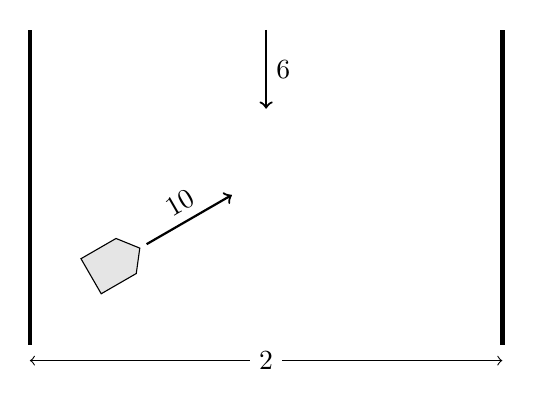
\begin{tikzpicture}
        %% Banks
        \draw[ultra thick] (-3,-2) -- (-3,2);
        \draw[ultra thick] (+3,-2) -- (+3,2);
        \draw[<->] (-3,-2.2) -- (+3,-2.2) node[pos=0.5,anchor=center,fill=white] {\SI{2}{\kilo\meter}};
        %% Boat
        \node[rotate=30,minimum size=0.5cm] (B) at (-2,-1) {};
        \draw[fill=white!90!black] (B.east) ++ (30:0.20) -- (B.south east) -- (B.south west) -- (B.north west) -- (B.north east) --cycle;
        \draw[thick,->] (B.east) ++(30:0.3) -- ++(30:1.25) node[pos=0.5,anchor=south,rotate=30] {\SI{10}{\kilo\meter\per\hour}};
        %% Current
        \draw[thick,->] (0,+2) -- (0,+1) node[pos=0.5,anchor=west] {\SI{6}{\kilo\meter\per\hour}};
    \end{tikzpicture}
    \end{center}
    If the speed of the water in the river is \SI{6}{\kilo\meter\per\hour},
        how much time is required for the crossing,
        assuming the boat is moving at its maximum speed?
    \begin{multicols}{3}
    \begin{choices}
      \correctchoice{\SI{0.25}{\hour}}
        \wrongchoice{\SI{0.10}{\hour}}
        \wrongchoice{\SI{0.35}{\hour}}
        \wrongchoice{\SI{0.40}{\hour}}
        \wrongchoice{\SI{0.50}{\hour}}
    \end{choices}
    \end{multicols}
\end{question}
}

\element{njctl}{
\begin{question}{kinematics-2d-q04}
    A projectile is fired from the surface of the Earth with a speed of \SI{200}{\meter\per\second} at an angle of \ang{45} above the horizontal.
    If the ground is level,
        what is the maximum height reached by the projectile?
    \begin{multicols}{3}
    \begin{choices}
      \correctchoice{\SI{1000}{\meter}}
        \wrongchoice{\SI{2000}{\meter}}
        \wrongchoice{\SI{3500}{\meter}}
        \wrongchoice{\SI{4000}{\meter}}
        \wrongchoice{\SI{5000}{\meter}}
    \end{choices}
    \end{multicols}
\end{question}
}

\element{njctl}{
\begin{question}{kinematics-2d-q05}
    A projectile is fired from the surface of the Earth with a speed $v_0$ at an angle of \ang{30} above the horizontal and hits a target at a range R from the starting point.
    If the ground is level,
        at what other angle above the horizontal could a second projectile be fired to hit the same target?
    \begin{multicols}{3}
    \begin{choices}
        \wrongchoice{\ang{30}}
        \wrongchoice{\ang{40}}
        \wrongchoice{\ang{45}}
      \correctchoice{\ang{60}}
        \wrongchoice{\ang{70}}
    \end{choices}
    \end{multicols}
\end{question}
}

\element{njctl}{
\begin{question}{kinematics-2d-q06}
    A rock is dropped from the top of \SI{80}{\meter} tower,
        and at the same time a ball is thrown from the top of the tower in a horizontal direction.
    Air resistance is negligible.
    The ball and the rock hit the level ground a distance of \SI{40}{\meter} apart.
    The horizontal velocity of the ball thrown was most nearly:
    \begin{multicols}{3}
    \begin{choices}
        \wrongchoice{\SI{5}{\meter\per\second}}
      \correctchoice{\SI{10}{\meter\per\second}}
        \wrongchoice{\SI{14}{\meter\per\second}}
        \wrongchoice{\SI{20}{\meter\per\second}}
        \wrongchoice{\SI{40}{\meter\per\second}}
    \end{choices}
    \end{multicols}
\end{question}
}

\element{njctl}{
\begin{question}{kinematics-2d-q07}
    At a particular instant,
        a student is on the ground sees a box falling with speed $v_1$ at an angle to the vertical.
    To a pilot flying horizontally at constant speed relative to the ground,
        the box appears to be falling vertically with a speed $v_2$ at that instant.
    What is the speed of the pilot relative to the ground?
    \begin{multicols}{2}
    \begin{choices}
        \wrongchoice{$v_1 + v_2$}
        \wrongchoice{$v_1 - v_2$}
        \wrongchoice{$v_2 - v_1$}
      \correctchoice{$\sqrt{v_1^2 - v_2^2}$}
        \wrongchoice{$\sqrt{v_1^2 + v_2^2}$}
    \end{choices}
    \end{multicols}
\end{question}
}

\element{njctl}{
\begin{question}{kinematics-2d-q08}
    A marble is fired from a spring-loaded gun straight up and reaches a maximum height $h$.
    The same gun is pointed at an angle of \ang{30} above the horizontal,
        what is the maximum height the marble can reach?
    \begin{multicols}{3}
    \begin{choices}
      \correctchoice{$\dfrac{h}{4}$}
        \wrongchoice{$\dfrac{3h}{2\sqrt{2}}$}
        \wrongchoice{$\dfrac{h}{2}$}
        \wrongchoice{$\dfrac{h}{\sqrt{2}}$}
        \wrongchoice{$h$}
    \end{choices}
    \end{multicols}
\end{question}
}

\newcommand{\njctlKinematicsTwoDQNine}{
\begin{tikzpicture}
    %% TODO: draw tikz
\end{tikzpicture}
}

\element{njctl}{
\begin{question}{kinematics-2d-q09}
    A marble is shot from ground level and follows a parabolic path as shown.
    Air resistance is neglible.
    Point $B$ is the highest point on the path.
    \begin{center}
        \njctlKinematicsTwoDQNine
    \end{center}
    Which best indicates the direction of the velocity, if any, of the marble at point $B$?
    \begin{multicols}{3}
    \begin{choices}
        %% NOTE: ANS is A
        \wrongchoice{
            \begin{tikzpicture}
                %% TODO: draw tikz
            \end{tikzpicture}
        }
        %% TODO: change to tikz, v=0
        \wrongchoice{The velocity is zero at point $B$.}
    \end{choices}
    \end{multicols}
\end{question}
}

\element{njctl}{
\begin{question}{kinematics-2d-q10}
    A marble is shot from ground level and follows a parabolic path as shown.
    Air resistance is neglible.
    Point $B$ is the highest point on the path.
    \begin{center}
        \njctlKinematicsTwoDQNine
    \end{center}
    Which of the following indicates the direction of the net acceleration of the marble at point $C$?
    \begin{multicols}{3}
    \begin{choices}
        %% NOTE: ANS is D
        \wrongchoice{
            \begin{tikzpicture}
                %% TODO: draw tikz
            \end{tikzpicture}
        }
    \end{choices}
    \end{multicols}
\end{question}
}

\element{njctl}{
\begin{question}{kinematics-2d-q11}
    A projectile is launched from the ground level and its initial velocity has two components: $v_{hor}$---horizontal component and $v_{ver}$---vertical component.
    Air resistance is negligible.
    When the projectile is at its highest,
        which of the following shows the vertical,
        horizontal components of its velocity and the vertical component of its acceleration?
    \begin{multicols}{3}
    \begin{choices}
        %% NOTE: ANS is E
        %% TODO: table options
        \wrongchoice{ }
        %Vertical
        %Horizontal
        %Acceleration
        %(A) v ver v hor 0
        %(B) v ver 0 0
        %(C) 0 v hor 0
        %(D) 0 0 g
        %(E) 0 v hor g
    \end{choices}
    \end{multicols}
\end{question}
}

\element{njctl}{
\begin{question}{kinematics-2d-q12}
    A target at point $X$ lies flat on the ground \SI{8}{\meter} from the side of a cliff that is \SI{20}{\meter} tall,
        as shown below.
    \begin{center}
    \begin{tikzpicture}
        %% TODO: draw tikz
    \end{tikzpicture}
    \end{center}
    A physics student rolls a ball off the horizontal cliff in the direction of the target. 
    Air resistance is negligible. 
    The horizontal speed with which the ball must leave the top of the cliff if it is to strike the target is:
    \begin{multicols}{3}
    \begin{choices}
      \correctchoice{\SI{4}{\meter\per\second}}
        \wrongchoice{\SI{6}{\meter\per\second}}
        \wrongchoice{\SI{12}{\meter\per\second}}
        \wrongchoice{\SI{20}{\meter\per\second}}
        \wrongchoice{\SI{24}{\meter\per\second}}
    \end{choices}
    \end{multicols}
\end{question}
}

\element{njctl}{
\begin{question}{kinematics-2d-q13}
    A physics student wants to hit a target with a rubber band ball from \SI{1.8}{\meter} away.
    If he throws the ball at a speed of \SI{6}{\meter\per\second} and the target is at the exact same height as where the ball is thrown,
        what angle from the horizontal must he throw the ball to hit the target?
    \begin{multicols}{3}
    \begin{choices}
        \wrongchoice{\ang{0}}
      \correctchoice{\ang{15}}
        \wrongchoice{\ang{30}}
        \wrongchoice{\ang{40}}
        \wrongchoice{\ang{45}}
    \end{choices}
    \end{multicols}
\end{question}
}

\element{njctl}{
\begin{question}{kinematics-2d-q14}
    An airplane pilot is moving with a velocity $v$ and drops a package. 
    In the absence of air resistance where is the package relative to the airplane at the moment it hits the ground?
    \begin{choices}
        \wrongchoice{Behind the airplane}
        \wrongchoice{In front of the airplane}
      \correctchoice{Directly below the airplane}
        \wrongchoice{Cannot be determined without knowing how height the plane is}
        \wrongchoice{Cannot be determined without knowing the distance traveled by the airplane.}
    \end{choices}
\end{question}
}

\element{njctl}{
\begin{question}{kinematics-2d-q15}
    At what angle must a student throw a ball in order to achieve its maximum distance?
    \begin{multicols}{3}
    \begin{choices}
        \wrongchoice{\ang{0}}
        \wrongchoice{\ang{30}}
      \correctchoice{\ang{45}}
        \wrongchoice{\ang{60}}
        \wrongchoice{\ang{90}}
    \end{choices}
    \end{multicols}
\end{question}
}

\element{njctl}{
\begin{question}{kinematics-2d-q16}
    %% Question 16-18
    The $x$ and $y$ coordinates of a particle in motion,
        as a function of time, are given:
    \begin{align*}
        x &= 8t^2 - 4t + 1\, , \\
        y &= 2t^3 - 3t^2 + 6t - 3\, ,
    \end{align*}
    where all quantities are in base SI units.
    %% start question
    The $x$ and $y$ components of the average velocity,
        in the interval from $t=\SI{0}{\second}$ to $t=\SI{3}{\second}$ are:
    \begin{choices}
        \wrongchoice{$v_x = \SI{36}{\meter\per\second}$,\phantom{$-$} $v_y = \SI{42}{\meter\per\second}$}
        \wrongchoice{$v_x = \SI{-20}{\meter\per\second}$,             $v_y = \SI{15}{\meter\per\second}$}
      \correctchoice{$v_x = \SI{20}{\meter\per\second}$,\phantom{$-$} $v_y = \SI{15}{\meter\per\second}$}
        \wrongchoice{$v_x = \SI{-36}{\meter\per\second}$,             $v_y = \SI{-42}{\meter\per\second}$}
        \wrongchoice{$v_x = \SI{25}{\meter\per\second}$,\phantom{$-$} $v_y = \SI{29}{\meter\per\second}$}
    \end{choices}
\end{question}
}

\element{njctl}{
\begin{question}{kinematics-2d-q17}
    %% Question 16-18
    The $x$ and $y$ coordinates of a particle in motion,
        as a function of time, are given:
    \begin{align*}
        x &= 8t^2 - 4t + 1\, , \\
        y &= 2t^3 - 3t^2 + 6t - 3\, ,
    \end{align*}
    where all quantities are in base SI units.
    %% start question
    The $x$ and $y$ components of the instantaneous velocity at $t= \SI{2}{\second}$ are:
    \begin{choices}
        \wrongchoice{$v_x = \SI{-24}{\meter\per\second}$,              $v_y = \SI{8}{\meter\per\second}$}
      \correctchoice{$v_x = \SI{28}{\meter\per\second}$,\phantom{$-$}  $v_y = \SI{18}{\meter\per\second}$}
        \wrongchoice{$v_x = \SI{20}{\meter\per\second}$,\phantom{$-$}  $v_y = \SI{15}{\meter\per\second}$}
        \wrongchoice{$v_x = \SI{-36}{\meter\per\second}$,              $v_y = \SI{42}{\meter\per\second}$}
        \wrongchoice{$v_x = \SI{12}{\meter\per\second}$,\phantom{$-$}  $v_y = \SI{8}{\meter\per\second}$}
    \end{choices}
\end{question}
}

\element{njctl}{
\begin{question}{kinematics-2d-q18}
    %% Question 16-18
    The $x$ and $y$ coordinates of a particle in motion,
        as a function of time, are given:
    \begin{align*}
        x &= 8t^2 - 4t + 1\, , \\
        y &= 2t^3 - 3t^2 + 6t - 3\, ,
    \end{align*}
    where all quantities are in base SI units.
    %% start question
    The $x$ and $y$ components of the instantaneous acceleration at $t=\SI{3}{\second}$ are:
    \begin{choices}
      \correctchoice{$a_x = \SI{16}{\meter\per\second\squared}$,              $a_y = \SI{30}{\meter\per\second\squared}$}
        \wrongchoice{$a_x = \SI{16}{\meter\per\second\squared}$,              $a_y = \SI{0}{\meter\per\second\squared}$}
        \wrongchoice{$a_x = \SI{0}{\meter\per\second\squared}$,\phantom{$0$}  $a_y = \SI{0}{\meter\per\second\squared}$}
        \wrongchoice{$a_x = \SI{16}{\meter\per\second\squared}$,              $a_y = \SI{8}{\meter\per\second\squared}$}
        \wrongchoice{$a_x = \SI{0}{\meter\per\second\squared}$,\phantom{$0$}  $a_y = \SI{30}{\meter\per\second\squared}$}
    \end{choices}
\end{question}
}

\element{njctl}{
\begin{question}{kinematics-2d-q19}
    Which of the following statements is true regarding ground-ground projectile motion?
    \begin{choices}
        \wrongchoice{$\left(v_x^2 + v_y^2\right)$ = constant.}
        \wrongchoice{Acceleration is $+g$ when the object is rising and $-g$ when falling.}
        \wrongchoice{In the absence of friction the acceleration depends on the object's mass}
        \wrongchoice{The velocity of the object is zero at the point of maximum elevation}
      \correctchoice{The horizontal motion is independent of the vertical motion}
    \end{choices}
\end{question}
}

\element{njctl}{
\begin{question}{kinematics-2d-q20}
    Two cannon balls are launched simultaneously off a cliff. 
    The two cannon balls have different masses and different horizontal initial velocities. 
    Which will strike the ground first?
    \begin{choices}
        \wrongchoice{The heaviest one}
        \wrongchoice{The lightest one}
        \wrongchoice{The slowest one}
        \wrongchoice{The fastest one }
      \correctchoice{They will strike the plane at the same time}
    \end{choices}
\end{question}
}

\element{njctl}{
\begin{question}{kinematics-2d-q21}
    The $x$ and $y$ coordinates of a particle in motion,
        as a function of time, are given:
    \begin{align*}
        x &= 5t^2 - 5t + 6\, , \\
        y &= 3t^3 - 2t^2 + 4t - 3 \, ,
    \end{align*}
    where all quantities are in base SI units.
    At the instant the $x$-component of velocity is equal to zero,
        the $y$-component of acceleration is:
    \begin{multicols}{3}
    \begin{choices}
      \correctchoice{\SI{5}{\meter\per\second\squared}}
        \wrongchoice{\SI{0.5}{\meter\per\second\squared}}
        \wrongchoice{\SI{2}{\meter\per\second\squared}}
        \wrongchoice{\SI{-10}{\meter\per\second\squared}}
        \wrongchoice{\SI{-5}{\meter\per\second\squared}}
    \end{choices}
    \end{multicols}
\end{question}
}

\element{njctl}{
\begin{question}{kinematics-2d-q22}
    Which of the following pairs of angles will result in the same maximum horizontal range of a projectile?
    \begin{multicols}{2}
    \begin{choices}
        \wrongchoice{$\theta_1=\ang{45}$, $\theta_2=\ang{30}$}
        \wrongchoice{$\theta_1=\ang{60}$, $\theta_2=\ang{45}$}
        \wrongchoice{$\theta_1=\ang{90}$, $\theta_2=\ang{30}$}
      \correctchoice{$\theta_1=\ang{30}$, $\theta_2=\ang{60}$}
        \wrongchoice{$\theta_1=\ang{75}$, $\theta_2=\ang{25}$}
    \end{choices}
    \end{multicols}
\end{question}
}

\newcommand{\njctlKinematicsTwoDQTwentyThree}{
\begin{tikzpicture}
    %% TODO: draw tikz
\end{tikzpicture}
}

\element{njctl}{
\begin{question}{kinematics-2d-q23}
    %% Questions 23-25
    A projectile is fired at time $t=\SI{0}{\second}$,
        from the edge of a cliff, with initial velocity components of $v_{ox}=\SI{30}{\meter\per\second}$ and $v_{oy}=\SI{50}{\meter\per\second}$.
    \begin{center}
        \njctlKinematicsTwoDQTwentyThree
    \end{center}
    %% start question
    The magnitude of the velocity at time $t=\SI{1}{\second}$ is:
    \begin{multicols}{3}
    \begin{choices}
        \wrongchoice{\SI{30}{\meter\per\second}}
        \wrongchoice{\SI{40}{\meter\per\second}}
      \correctchoice{\SI{50}{\meter\per\second}}
        \wrongchoice{\SI{70}{\meter\per\second}}
        \wrongchoice{\SI{90}{\meter\per\second}}
    \end{choices}
    \end{multicols}
\end{question}
}

\element{njctl}{
\begin{question}{kinematics-2d-q24}
    %% Questions 23-25
    A projectile is fired at time $t=\SI{0}{\second}$,
        from the edge of a cliff, with initial velocity components of $v_{ox}=\SI{30}{\meter\per\second}$ and $v_{oy}=\SI{50}{\meter\per\second}$.
    \begin{center}
        \njctlKinematicsTwoDQTwentyThree
    \end{center}
    %% start question
    The velocity at the highest point is:
    \begin{multicols}{3}
    \begin{choices}
        \wrongchoice{\SI{50}{\meter\per\second}}
        \wrongchoice{\SI{40}{\meter\per\second}}
        \wrongchoice{\SI{60}{\meter\per\second}}
      \correctchoice{\SI{30}{\meter\per\second}}
        \wrongchoice{\SI{10}{\meter\per\second}}
    \end{choices}
    \end{multicols}
\end{question}
}

\element{njctl}{
\begin{question}{kinematics-2d-q25}
    %% Questions 23-25
    A projectile is fired at time $t=\SI{0}{\second}$,
        from the edge of a cliff, with initial velocity components of $v_{ox}=\SI{30}{\meter\per\second}$ and $v_{oy}=\SI{50}{\meter\per\second}$.
    \begin{center}
        \njctlKinematicsTwoDQTwentyThree
    \end{center}
    %% start question
    The magnitude of the acceleration at the highest point is:
    \begin{multicols}{3}
    \begin{choices}
        \wrongchoice{zero}
        \wrongchoice{\SI{3.7}{\meter\per\second\squared}}
        \wrongchoice{\SI{1.7}{\meter\per\second\squared}}
        \wrongchoice{\SI{4.9}{\meter\per\second\squared}}
      \correctchoice{\SI{9.8}{\meter\per\second\squared}}
    \end{choices}
    \end{multicols}
\end{question}
}

\element{njctl}{
\begin{question}{kinematics-2d-q26}
    The acceleration of a particle is given by the equation: $a(t) = 12t - 8$.
    Given that $v_0=0$,
        at what time does the particle come to rest?
    \begin{multicols}{3}
    \begin{choices}
        \wrongchoice{\SI{1/2}{\second}}
        \wrongchoice{\SI{3/4}{\second}}
        \wrongchoice{\SI{2/3}{\second}}
      \correctchoice{\SI{4/3}{\second}}
        \wrongchoice{\SI{12}{\second}}
    \end{choices}
    \end{multicols}
\end{question}
}

\element{njctl}{
\begin{question}{kinematics-2d-q27}
    %% Questions 27-28
    An object is launched with an initial velocity of 10 meters per second from the ground level at an angle of \ang{53} above the horizontal.
    %% start question
    What are the horizontal and vertical components of the ball's velocity at the beginning of its flight?
    \begin{choices}
      \correctchoice{$v_x=\SI{6}{\meter\per\second}$,  $v_y=\SI{8}{\meter\per\second}$}
        \wrongchoice{$v_x=\SI{5}{\meter\per\second}$,  $v_y=\SI{5}{\meter\per\second}$}
        \wrongchoice{$v_x=\SI{10}{\meter\per\second}$, $v_y=\SI{10}{\meter\per\second}$}
        \wrongchoice{$v_x=\SI{8}{\meter\per\second}$,  $v_y=\SI{6}{\meter\per\second}$}
        \wrongchoice{$v_x=\SI{0}{\meter\per\second}$,  $v_y=\SI{10}{\meter\per\second}$}
    \end{choices}
\end{question}
}

\element{njctl}{
\begin{question}{kinematics-2d-q28}
    %% Questions 27-28
    An object is launched with an initial velocity of 10 meters per second from the ground level at an angle of \ang{53} above the horizontal.
    %% start question
    What are the horizontal and vertical components of the ball's velocity at the apex of its flight?
    \begin{choices}
        \wrongchoice{$v_x=\SI{6}{\meter\per\second}$, $v_y=\SI{8}{\meter\per\second}$}
      \correctchoice{$v_x=\SI{6}{\meter\per\second}$, $v_y=\SI{0}{\meter\per\second}$}
        \wrongchoice{$v_x=\SI{0}{\meter\per\second}$, $v_y=\SI{0}{\meter\per\second}$}
        \wrongchoice{$v_x=\SI{8}{\meter\per\second}$, $v_y=\SI{6}{\meter\per\second}$}
        \wrongchoice{$v_x=\SI{8}{\meter\per\second}$, $v_y=\SI{0}{\meter\per\second}$}
    \end{choices}
\end{question}
}

\element{njctl}{
\begin{question}{kinematics-2d-q29}
    The $x$ and $y$ components of a particle's acceleration is given as a function of time, are
    \begin{align*}
        a_x &= -4t + 1\, , \\
        a_y &= 2t + 3 \, ,
    \end{align*}
    with all quantities are in base SI units.
    What is the magnitude of the particle's velocity at $t=\SI{1}{\second}$ if its initial velocity is equal to zero?
    \begin{multicols}{3}
    \begin{choices}
      \correctchoice{\SI{4.1}{\meter\per\second}}
        \wrongchoice{\SI{2.1}{\meter\per\second}}
        \wrongchoice{\SI{5.3}{\meter\per\second}}
        \wrongchoice{\SI{-2.1}{\meter\per\second}}
        \wrongchoice{\SI{-5.0}{\meter\per\second}}
    \end{choices}
    \end{multicols}
\end{question}
}

\element{njctl}{
\begin{question}{kinematics-2d-q30}
    A projectile is launched from the ground level in two trials,
        first at a \ang{20} and the second at a \ang{70} above the horizontal. 
    They both land on the ground. 
    How would you compare the maximum height and the time in the air of the projectiles?
    \begin{choices}
        %% TODO: table
        %% Maximum Height Time in Air
        \wrongchoice{H 20 < H 70,  t 20 > t 70}
        \wrongchoice{H 20 = H 70,  t 20 = t 70}
        \wrongchoice{H 20 > H 70, t 20 > t 70}
        \wrongchoice{H 20 > H 70, t 20 < t 70}
      \correctchoice{H 20 < H 70, t 20 < t 70}
    \end{choices}
\end{question}
}

\element{njctl}{
\begin{question}{kinematics-2d-q31}
    An object moves in a straight line and experiences an acceleration given by the formula $a=-2t$.
    At time $t=0$ object's velocity is \SI{4}{\meter\per\second} in the positive direction. 
    At what time does the object instantaneously come to rest?
    \begin{multicols}{2}
    \begin{choices}
      \correctchoice{\SI{2}{\second}}
        \wrongchoice{\SI{4}{\second}}
        \wrongchoice{\SI{5}{\second}}
        \wrongchoice{\SI{6}{\second}}
        \wrongchoice{It never comes to rest}
    \end{choices}
    \end{multicols}
\end{question}
}

\element{njctl}{
\begin{question}{kinematics-2d-q32}
    A toy car starts from rest and accelerates on a flat horizontal surface. 
    At time $t=\text{zero}$ its velocity $v_0=\text{zero}$.
    The car's acceleration is given by formula:
    \begin{equation*}
        \vec{a} = \left(\SI{2}{\meter\per\second}\right)\hat{\imath} + \left(\SI{1}{\meter\per\second}\right)\hat{\jmath}\, .
    \end{equation*}
    What is the $x$-coordinate of the particle when its $y$-coordinate is \SI{10}{\meter\per\second}?
    \begin{multicols}{3}
    \begin{choices}
        \wrongchoice{\SI{10}{\meter}}
      \correctchoice{\SI{20}{\meter}}
        \wrongchoice{\SI{40}{\meter}}
        \wrongchoice{\SI{60}{\meter}}
        \wrongchoice{\SI{80}{\meter}}
    \end{choices}
    \end{multicols}
\end{question}
}

\element{njctl}{
\begin{question}{kinematics-2d-q33}
    The velocity as a function of time of a moving particle is given by formula:
    \begin{equation*}
        v = \dfrac{1}{\alpha} v_0 \mathrm{e}^{-\alpha t} \,,
    \end{equation*}
    where $v_0$ and $\alpha$ are constants, and all quantitites are in SI units. 
    What is the acceleration of the particle as a function of time?
    \begin{multicols}{2}
    \begin{choices}
        \wrongchoice{$a = \dfrac{1}{\alpha} v_0 \mathrm{e}^{-\alpha t}$}
        \wrongchoice{$a = v_0 \mathrm{e}^{-\alpha t}$}
        \wrongchoice{$a = -v_0 \mathrm{e}^{-\alpha t}$}
        \wrongchoice{$a = \alpha v_0 \mathrm{e}^{-\alpha t}$}
      \correctchoice{$a = -\alpha v_0 \mathrm{e}^{-\alpha t}$}
    \end{choices}
    \end{multicols}
\end{question}
}

\newcommand{\njctlKinematicsTwoDQThirtyFour}{
\begin{tikzpicture}
    %% TODO: pgfplots
\end{tikzpicture}
}

\newcommand{\njctlKinematicsTwoDQThirtyFourA}{
\begin{tikzpicture}
    %% TODO: pgfplots
\end{tikzpicture}
}

\element{njctl}{
\begin{question}{kinematics-2d-q34}
    A projectile is fired from the ground level at an angle $\theta$ above the horizontal. 
    \begin{center}
        \njctlKinematicsTwoDQThirtyFour
    \end{center}
    Which of the following graphs represents the vertical component of the projectile’s velocity as a function of time? 
    Air resistance is negligible.
    \begin{multicols}{2}
    \begin{choices}
        \AMCboxDimensions{down=-1.5em}
        %% NOTE: ANS is D
        %% TODO: \newcommand options
        \wrongchoice{
            \njctlKinematicsTwoDQThirtyFourA
        }
    \end{choices}
    \end{multicols}
\end{question}
}

\element{njctl}{
\begin{question}{kinematics-2d-q35}
    A projectile is fired from the ground level at an angle $\theta$ above the horizontal. 
    \begin{center}
        \njctlKinematicsTwoDQThirtyFour
    \end{center}
    Which of the following graphs represents the vertical component of the projectile's acceleration as a function of time? 
    Air resistance is negligible.
    \begin{multicols}{2}
    \begin{choices}
        \AMCboxDimensions{down=-1.5em}
        %% NOTE: ANS is A
        %% TODO: \newcommand options
        \wrongchoice{
            \njctlKinematicsTwoDQThirtyFourA
        }
    \end{choices}
    \end{multicols}
\end{question}
}

\element{njctl}{
\begin{question}{kinematics-2d-q36}
    Which of the following pairs of equations can describe the trajectory of projectile motion?
    \begin{multicols}{2}
    \begin{choices}
        \wrongchoice{$x = \alpha t$,        $y = \beta t$}
        \wrongchoice{$x = \alpha t^2$,      $y = \beta t^2$}
      \correctchoice{$x = \alpha t$,        $y = \beta t^2$}
        \wrongchoice{$x = \alpha \sqrt{t}$, $y = \beta\sqrt{t}$}
        \wrongchoice{$x = \dfrac{\alpha}{\sqrt{t}}$, $y = \dfrac{\beta}{\sqrt{t}}$}
    \end{choices}
    \end{multicols}
\end{question}
}

\element{njctl}{
\begin{question}{kinematics-2d-q37}
    A projectile is launched from the ground with an initial velocity $v_0$ at an angle $\theta$ above the horizontal. 
    How long will the projectile remain in air?
    \begin{multicols}{2}
    \begin{choices}
        \wrongchoice{$\dfrac{v_0\sin\theta}{g}$}
      \correctchoice{$\dfrac{2v_0\sin\theta}{g}$}
        \wrongchoice{$\dfrac{v_0\cos\theta}{g}$}
        \wrongchoice{$\dfrac{2v_0\cos\theta}{g}$}
        \wrongchoice{$\dfrac{v_0\tan\theta}{g}$}
    \end{choices}
    \end{multicols}
\end{question}
}

\element{njctl}{
\begin{question}{kinematics-2d-q38}
    A projectile is launched from the ground with an initial velocity $v_0$ at an angle $\theta$ above the horizontal. 
    How long will it take the projectile to reach the maximum height?
    \begin{multicols}{2}
    \begin{choices}
      \correctchoice{$\dfrac{2v_0\sin\theta}{g}$}
        \wrongchoice{$\dfrac{v_0\cos\theta}{g}$}
        \wrongchoice{$\dfrac{2v_0\cos\theta}{g}$}
        \wrongchoice{$\dfrac{v_0\tan\theta}{g}$}
        \wrongchoice{$\dfrac{v_0\sin\theta}{g}$}
    \end{choices}
    \end{multicols}
\end{question}
}

\element{njctl}{
\begin{question}{kinematics-2d-q39}
    A projectile is launched from the ground with an initial velocity $v_0$ at an angle $\theta$ above the horizontal. 
    What is the maximum height of the projectile?
    \begin{multicols}{2}
    \begin{choices}
        \wrongchoice{$\dfrac{v_0^2\sin\theta^2}{g}$}
        \wrongchoice{$\dfrac{2v_0^2\sin\theta^2}{g}$}
      \correctchoice{$\dfrac{v_0^2\sin\theta^2}{2g}$}
        \wrongchoice{$\dfrac{v_0^2\cos\theta^2}{2g}$}
        \wrongchoice{$\dfrac{v_0^2\cos\theta^2}{g}$}
    \end{choices}
    \end{multicols}
\end{question}
}

\element{njctl}{
\begin{question}{kinematics-2d-q40}
    A projectile is launched from the ground with an initial velocity $v_0$ at an angle $\theta$ above the horizontal. 
    What is the maximum horizontal range of the projectile?
    \begin{multicols}{2}
    \begin{choices}
        \wrongchoice{$\dfrac{v_0^2\sin 2\theta}{g}$}
        \wrongchoice{$\dfrac{2v_0^2\cot 2\theta}{g}$}
        \wrongchoice{$\dfrac{v_0^2\cos 2\theta}{g}$}
      \correctchoice{$\dfrac{v_0^2\sin 2\theta}{g}$}
        \wrongchoice{$\dfrac{v_0^2\tan 2\theta}{g}$}
    \end{choices}
    \end{multicols}
\end{question}
}


%% ANSWERS:
%% 1.C 2.E 3.A 4.A 5.D 6.B 7.D 8.A 9.A 10.D 11.E 12.A 13.B 14.C 15.C 16.C 17.B 18.A 19.E 20.E 21.A 22.D 23.C 24.D 25.E 26.D 27.A 28.B 29.A 30.E 31.A 32.B 33.E 34.D 35.A 36.C 37.B 38.A 39.C 40.D


\endinput


